
\documentclass[22pt]{beamer}

\usetheme{Warsaw}
\usepackage{multirow}
\usepackage[numbers]{natbib}
\title{Introduction to Version Control with Git \cite{loeliger2012version}}

\author{Khaled El-Wazan \thanks{khaled\_elwazan@alex-sci.edu.eg}}

\institute{Department of Mathematics and Computer Science, Faculty of Science, Alexandria University}

\date{}

\AtBeginSection[]{
  \begin{frame}
  \vfill
  \centering
  \begin{beamercolorbox}[sep=8pt,center,shadow=true,rounded=true]{title}
    \usebeamerfont{title} \thesection: \insertsectionhead\par%
  \end{beamercolorbox}
  \vfill
  \end{frame}
}

\setbeamertemplate{caption}[numbered]

% remove headlines at a certain frame

\makeatletter
    \newenvironment{withoutheadline}{
        \setbeamertemplate{headline}[default]
        \def\beamer@entrycode{\vspace*{-\headheight}}
    }{}
\makeatother
\begin{document}
\Large
\maketitle


\begin{frame}
    \frametitle{Outlines}
    \tableofcontents
\end{frame}


\section{Background}

\begin{frame}
    \frametitle{Background}
    \begin{enumerate}
        \item A wise man strategies.
        \item Text and code projects need back up plans.
        \item The main issues with projects.
        \item Version control to the rescue.


              \pause
        \item Develop and maintain a repository of content, provide access to historical editions
              of each datum, and record all changes in a log.
    \end{enumerate}
    \pause
    \begin{definition}
        A tool that manages and tracks different versions of software or other content is referred
        to generically as a version control system (VCS).
    \end{definition}

\end{frame}


\section{History}
\begin{frame}
    \frametitle{Histroy}
    \begin{itemize}
        \item Discords between tools and projects.
        \item The temptation of creating tools on the fly.
        \item Git, the information manager from hell.
        \item The genesis of Git.
        \item BitKeeper, free as in beer.
    \end{itemize}


\end{frame}

\section{Main and Essential Features}
\begin{frame}
    \frametitle{The Elusive Features}
    \begin{itemize}
        \item Facilitate Distributed Development.
              \pause
        \item Scale to Handle Thousands of Developers.
              \pause
        \item Perform Quickly and Efficiently.
              \pause
        \item Maintain Integrity and Trust.
              \pause
        \item Enforce Accountability.
              \pause
        \item Immutability.
              \pause
        \item Atomic Transactions.
              \pause
        \item Support and Encourage Branched Development.
              \pause
        \item Complete Repositories.
              \pause
        \item A Clean Internal Design.
              \pause
        \item Be Free, as in Freedom.
    \end{itemize}



\end{frame}

\section{The First of Many}

\begin{frame}[allowframebreaks]
    \frametitle{The First Commit}

    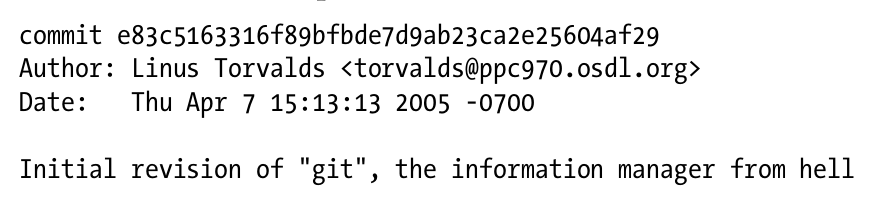
\includegraphics[width=\linewidth]{images/Screenshot from 2020-12-10 13-43-08.png}
    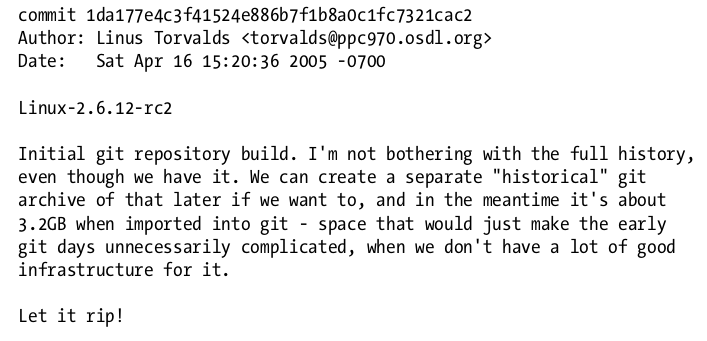
\includegraphics[width=\linewidth]{images/Screenshot from 2020-12-10 13-35-57.png}


\end{frame}

\section{The Bibliography}
\begin{frame}[allowframebreaks]
    \frametitle{References}
    \bibliographystyle{IEEEtranN}
    \bibliography{references}
\end{frame}


\end{document}